\section{Numerical Tests}
\label{sec:numerical}

\subsection{Problems with Known Smooth Solutions}
\label{sec:smoothProblems}

To compare the accuracy of the IMEX schemes, we present results from smooth problems in streaming, absorption, and scattering dominated regimes in one spatial dimension.  
For all tests in this subsection, we use third order accurate spatial discretization (polynomials of degree $k=2$) and we employ the maximum entropy closure in the low occupancy limit (i.e., the Minerbo closure).  
We compare results obtained using IMEX schemes proposed here (PA2+ and PARSD) with IMEX schemes from Hu et al. \cite{hu_etal_2017} (PA2), McClarren et al. \cite{mcclarren_etal_2008} (PC2), Pareschi \& Russo \cite{pareschiRusso_2005} (SSP2332), and Cavaglieri \& Bewley \cite{cavaglieriBewley2015} (RKCB2).  
In the streaming test, we also include results obtained with second-order and third-order accurate explicit strong stability-preserving Runge-Kutta methods \cite{gottlieb_etal_2001} in the comparison (SSPRK2 and SSPRK3, respectively).  
See \ref{app:butcherTables} for further details.  
The time step is set to $\dt=0.1\times\dx$.  

When comparing the numerical results to analytic solutions, errors are computed in the $L^{1}$-error norm.  
We compare results either in the absolute error ($E_{\mbox{\tiny Abs}}^{1}$) or the relative error ($E_{\mbox{\tiny Rel}}^{1}$), defined for a scalar quantity $u_{h}$ (approximating $u$) as
\begin{equation}
  E_{\mbox{\tiny Abs}}^{1}[u_{h}](t)
  =\f{1}{|D|}\sum_{\bK\in\mathscr{T}}\int_{\bK}|u_{h}(\vect{x},t)-u(\vect{x},t)|\,d\vect{x}
  \label{eq:errorNormAbsolute}
\end{equation}
and
\begin{equation}
  E_{\mbox{\tiny Rel}}^{1}[u_{h}](t)
  =\f{1}{|D|}\sum_{\bK\in\mathscr{T}}\int_{\bK}|u_{h}(\vect{x},t)-u(\vect{x},t)|/|u(\vect{x},t)|\,d\vect{x},
  \label{eq:errorNormRelative}
\end{equation}
respectively.  
The integrals in Eqs.~\eqref{eq:errorNormAbsolute} and \eqref{eq:errorNormRelative} are computed with a $3$-point Gaussian quadrature.  

\subsubsection{Sine Wave: Streaming}

The first test involves the streaming part only, and does not include any collisions ($\sigma_{\Ab}=\sigma_{\Scatt}=0$).  
We consider a periodic domain $D=\{x:x\in[0,1]\}$, and let the initial condition be given by
\begin{equation}
  \cJ(x,t=0)=\cH_{x}(x,t=0)=0.5+0.49\times\sin\big(2\pi\,x\big).  
  \label{eq:initialConditionStreaming}
\end{equation}
We evolve until $t=10$, when the sine wave has completed 10 crossings of the computational domain.  
We vary the number of elements ($N$) from $8$ to $128$ and compute errors for various time stepping schemes.  

In Figure~\ref{fig:SineWaveStreaming}, the absolute error for the number density $E_{\mbox{\tiny Abs}}^{1}[\cJ_{h}](t=10)$ is plotted versus $N$ (see figure caption for details).  
Errors obtained with SSPRK3 are smallest and decrease as $N^{-3}$ (cf. bottom black dash-dot reference line), as expected for a scheme combining third-order accurate time stepping with third-order accurate spatial discretization.  
For all the other schemes, using second-order accurate explicit time stepping, the error decreases as $N^{-2}$.  
Among the second-order accurate methods, SSP2332 has the smallest error, followed by RKCB2.  
Errors for the remaining schemes (including SSPRK2) are indistinguishable on the plot.  
\begin{figure}[h]
  \centering
    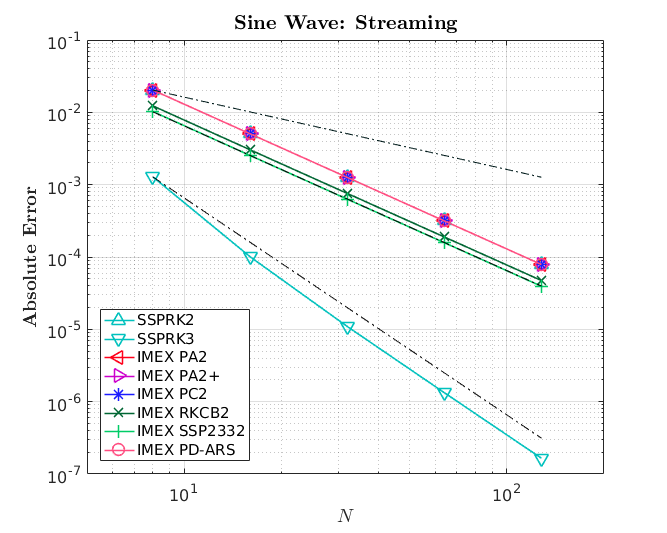
\includegraphics[width=\textwidth]{figures/SineWaveStreaming}
   \caption{Absolute error (cf. Eq.~\eqref{eq:errorNormAbsolute}) versus number of elements $N$ for the streaming sine wave test.  Results employing various time stepping schemes are compared: SSPRK2 (cyan triangles pointing up), SSPRK3 (cyan triangles pointing down), PA2 (red), PA2+ (purple), PC2 (blue), RKCB2 (dark green), SSP2332 (green), and PARSD (light red circles).  Black dash-dot reference lines are proportional to $N^{-1}$ (top), $N^{-2}$ (middle), and $N^{-3}$ (bottom), respectively.}
  \label{fig:SineWaveStreaming}
\end{figure}


\subsubsection{Sine Wave: Damping}

The next test we consider, adapted from \cite{skinnerOstriker_2013}, consists of a sine wave propagating with unit speed in a purely absorbing medium ($f_{0}=0$, $\sigma_{\Scatt}=0$), which results in exponential damping of the wave amplitude.  
We consider a periodic domain $D=\{x:x\in[0,1]\}$, and let the initial condition ($t=0$) be given as in Eq.~\eqref{eq:initialConditionStreaming}.  
For a constant absorption opacity $\sigma_{\Ab}$, the analytical solution at $t>0$ is given by
\begin{equation}
  \cJ(x,t)=\cJ_{0}(x-t)\times\exp(-\sigma_{\Ab} t)
  \quad\text{and}\quad
  \cH_{x}(x,t)=\cJ(x,t),
\end{equation}
where $\cJ_{0}(x)=\cJ(x,0)$.  

We compute numerical solutions for three values of the absorption opacity ($\sigma_{\Ab}=0.1$, $1$, and $10$), and adjust the end time $t_{\mbox{\tiny end}}$ so that $\sigma_{\Ab}t_{\mbox{\tiny end}}=10$, and the initial condition has been damped by factor $e^{-10}$.  
Thus, for $\sigma_{\Ab}=0.1$ the sine wave crosses the domain 100 times, while for $\sigma_{\Ab}=10$, it crosses the grid once.  

Figure~\ref{fig:SineWaveDamping} shows convergence results, obtained using different values of $\sigma_{\Ab}$, for various IMEX schemes at $t=t_{\mbox{\tiny end}}$.  
Results for $\sigma_{\Ab}=0.1$, $1$, and $10$ are plotted with red, green, and blue lines, respectively (see figure caption for further details).  
All the second-order accurate schemes (PA2, PA2+, RKCB2, and SSP2332) display second-order accurate convergence rates (cf. bottom, black dash-dot reference line).  
For $\sigma_{\Ab}=0.1$, SSP2332 is the most accurate among these schemes, while PA2+ is the most accurate for $\sigma_{\Ab}=10$.  
On the other hand, PC2 and PARSD are indistinguishable and display at most first-order accurate convergence, as expected.  
(For $\sigma_{\Ab}=0.1$, PC2 and PARSD are the most accurate schemes for $N=8$ and $N=16$.)

\begin{figure}[h]
  \centering
    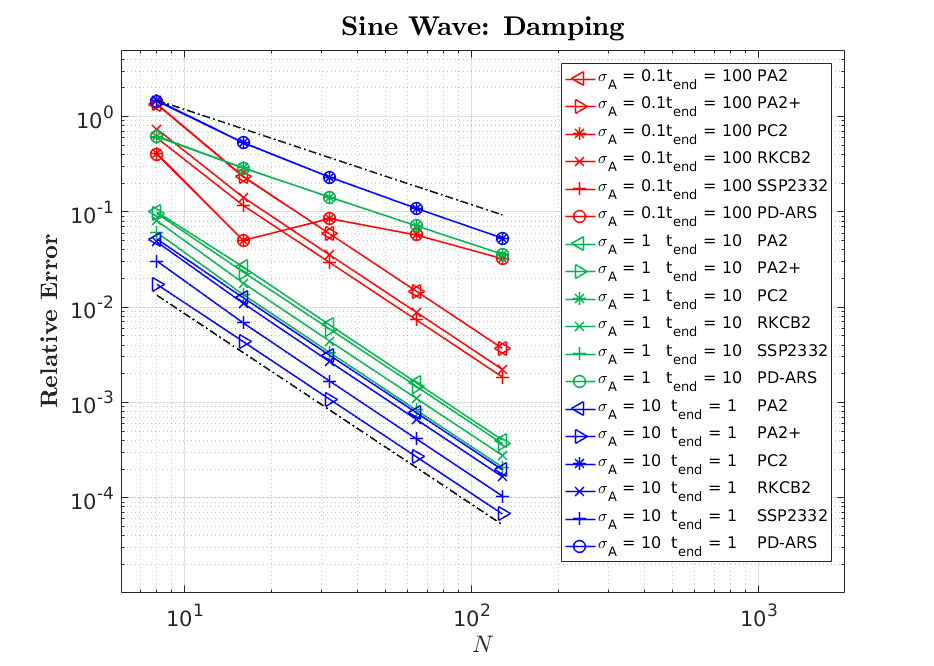
\includegraphics[width=\textwidth]{figures/SineWaveDamping}
   \caption{Relative error (cf. Eq.~\eqref{eq:errorNormRelative}) versus number of elements for the damping sine wave test.  Results for different values of the absorption opacity $\sigma_{\Ab}$, employing various IMEX time stepping schemes, are compared.  Errors for $\sigma_{\Ab}=0.1$, $1$, and $10$ are plotted with red, green, and blue lines, respectively.  The IMEX schemes employed are: PA2 (triangles pointing left), PA2+ (triangles pointing right), PC2 (asterisk), RKCB2 ($\times$), SSP2332 ($+$), and PARSD (circles).  Black dash-dot reference lines are proportional to $N^{-1}$ (top) and $N^{-2}$ (bottom), respectively.}
  \label{fig:SineWaveDamping}
\end{figure}

\subsubsection{Sine Wave: Diffusion}

The final test with known smooth solutions, adopted from \cite{radice_etal_2013}, is diffusion of a sine wave in a purely scattering medium ($f_{0}=0$, $\sigma_{\Ab}=0$).  
The computational domain $D=\{x:x\in[-3,3]\}$ is periodic, and the initial condition is given by
\begin{equation}
  \cJ_{0}(x)=0.5+0.49\times\sin\big(\pi\,x/3\big)
  \quad\text{and}\quad
  \cH_{x,0}
  =-\f{1}{3\sigma_{\Scatt}}\pderiv{\cJ_{0}}{x}.  
  \label{eq:initialConditionDiffusion}
\end{equation}
For a sufficiently high scattering opacity, the moment equations limit to a diffusion equation for the number density (deviations appear at the $1/\sigma_{\Scatt}^{2}$-level).  
With the initial conditions in Eq.~\eqref{eq:initialConditionDiffusion}, the analytical solution to the limiting diffusion equation is given by
\begin{equation}
  \cJ(x,t)=\cJ_{0}(x)\times\exp\big(-\pi^{2}\,t/(27\,\sigma_{\Scatt})\big),
\end{equation}
and $\cH_{x}=(3\,\sigma_{\Scatt})^{-1}\pd{\cJ}{x}$.  
When computing errors for this test, we compare the numerical results obtained with the two-moment model to the analytical solution to the limiting diffusion equation.  
We compute numerical solutions using three values of the scattering opacity ($\sigma_{\Scatt}=10^{2}$, $10^{3}$, and $10^{4}$), and adjust the end time so that $t_{\mbox{\tiny end}}/\sigma_{\Scatt}=1$.  
The initial amplitude of the sine wave has then been reduced by a factor $e^{-\pi^{2}/27}\approx0.694$ for all values of $\sigma_{\Scatt}$.  

\begin{figure}[h]
  \centering
  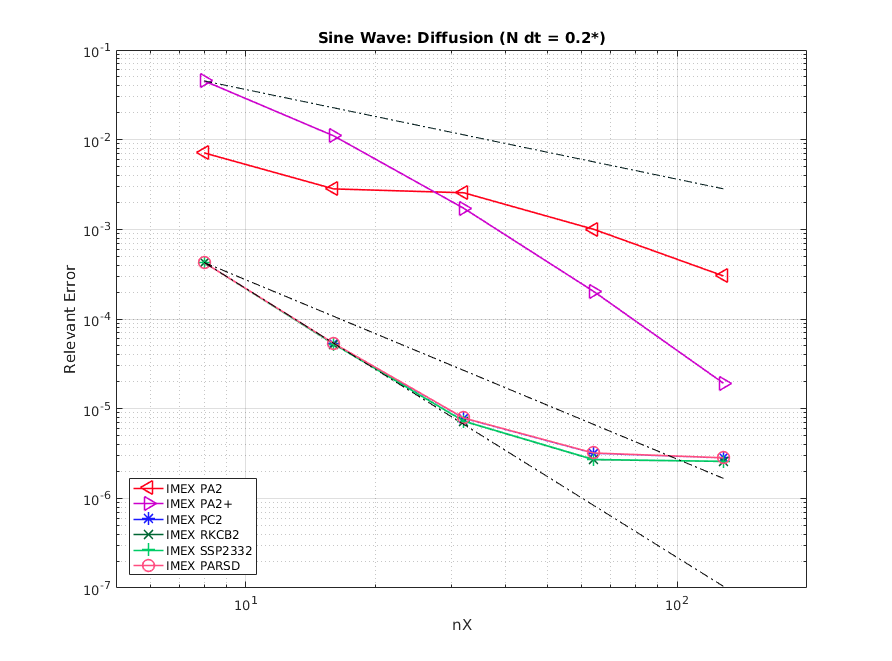
\includegraphics[width=1.0\textwidth]{figures/SineWaveDiffusionN}
   \caption{Absolute error (cf. Eq.~\eqref{eq:errorNormAbsolute}) for the number density $\cJ$ versus number of elements for the sine wave diffusion test.  Results with different values of the scattering opacity $\sigma_{\Scatt}$, employing different IMEX schemes, are compared.  Errors with $\sigma_{\Scatt}=10^{2}$, $10^{3}$, and $10^{4}$ are plotted with red, green, and blue lines, respectively.  The IMEX schemes employed are: PA2 (triangle pointing left), PA2+ (triangle pointing right), PC2 (asterisk), RKCB2 (cross), SSP2332 (plus), and PARSD (circle).  Black dash-dot reference lines are proportional to $N^{-1}$ (top) and $N^{-2}$ (bottom), respectively.}
  \label{fig:SineWaveDiffusionJ}
\end{figure}

\begin{figure}[h]
  \centering
  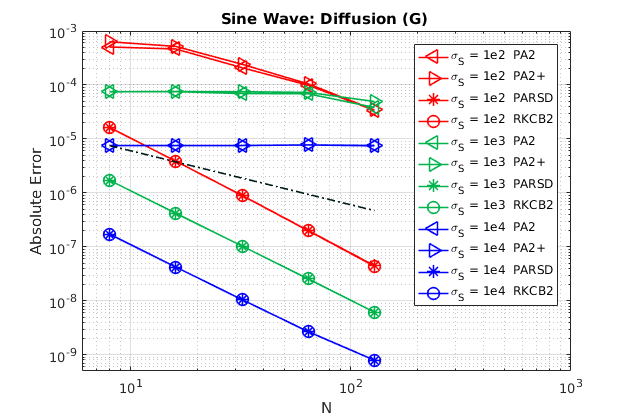
\includegraphics[width=1.0\textwidth]{figures/SineWaveDiffusionG}
   \caption{Same as in Figure~\ref{fig:SineWaveDiffusionJ}, but for the number flux $\cH_{x}$.}
  \label{fig:SineWaveDiffusionH}
\end{figure}

In Figures~\ref{fig:SineWaveDiffusionJ} and \ref{fig:SineWaveDiffusionJ} we plot the absolute error, obtained using different values of $\sigma_{\Scatt}$, for various IMEX schemes at $t=t_{\mbox{\tiny end}}$.  
Results for $\sigma_{\Scatt}=10^{2}$, $10^{3}$, and $10^{4}$ are plotted with red, green, and blue lines, respectively (see figure caption for further details).  
(Scheme PC2 has been shown to work well for this test \cite{radice_etal_2013}, but is included here for comparison with the other IMEX schemes.)
Schemes PARSD, RKCB2, and SSP2332 are accurate for this test, and display third-order accuracy for the number density $\cJ$ and second-oder accuracy for $\cH_{x}$.  
For $\sigma=10^{2}$, the errors do not drop below $10^{-6}$ because of differences between the two-moment model and the diffusion equation used to obtain the analytic solution.  
For larger values of the scattering opacity, the two-moment model agrees better with the diffusion model, and we observe convergence over the entire range of $N$.  
Schemes PA2 and PA2+ do not perform well on this test (for reasons discussed in Section~\ref{sec:imex}).  
For $\sigma_{\Scatt}=10^{2}$, errors in $\cJ$ and $\cH_{x}$ decrease with increasing $N$, but for $\sigma_{\Scatt}=10^{4}$, errors remain constant with increasing $N$ over the entire range.  

\subsection{Packed Beam}

Next we consider a one-dimensional test with discontinuous initial conditions.  
The purpose of this test is to further gauge the accuracy of the two-moment model and demonstrate the robustness of the DG scheme for dynamics close to the boundary of the realizable set $\cR$.  
The computational domain is $D=\{x:x\in[-1,1]\}$, and the initial condition is obtained from a distribution function given by
\begin{equation}
  f(x,\mu)
  =\left\{
  \begin{array}{cl}
    1        & \text{if} ~ x\le x_{\mbox{\tiny D}}, ~ \mu\ge\mu_{\mbox{\tiny D}} \\
    \delta & \text{if} ~ x\le x_{\mbox{\tiny D}}, ~ \mu<   \mu_{\mbox{\tiny D}} \\
    \delta & \text{otherwise},
  \end{array}
  \right.
\end{equation}
so that, with $\mu_{\mbox{\tiny D}}=0$, $\vect{\cM}\equiv\vect{\cM}_{\mbox{\tiny L}}=\big(0.5\,(1+\delta),0.25\,(1-\delta)\big)^{T}$ for $x\le x_{\mbox{\tiny D}}$, and $\vect{\cM}\equiv\vect{\cM}_{\mbox{\tiny R}}=\big(\delta,0\big)^{T}$ for $x> x_{\mbox{\tiny D}}$, where $\delta>0$ is a small parameter ($\delta\ll1$).  
We let $\delta=10^{-8}$, so that the initial conditions are very close to the boundary of the realizable domain (cf. Figure~\ref{fig:RealizableSetFermionic}).  
The analytical solution can be easily obtained by solving the transport equation for all angles $\mu$ (independent linear advection equations), and taking the angular moments.  
The numerical results shown in this section were obtained with the third-order scheme (polynomials of degree $k=2$ and the SSPRK3 time stepper) using $400$ elements.  
The time step is set to $\dt=0.1\times\dx$

Figure~\ref{fig:PackedBeam} shows results for various times obtained with the two-moment model.  
In the upper panels we plot the number density, while the number flux density is plotted in the lower panels.  
Numerical solutions are plotted with solid lines, while the analytical solution is plotted with dashed lines.  
In the left panels, the algebraic maximum entropy closure of Cernohorsky \& Bludman (CB) \cite{cernohorskyBludman_1994} (cf. Eqs.~\eqref{eq:eddingtonFactor} and \eqref{eq:closureMECB}) was used, while in the right panels the Minerbo closure (cf. Eqs.~\eqref{eq:eddingtonFactorLow} and \eqref{eq:closureMECB}) was used.  
For this test, the use of the realizability-preserving limiter described in Section~\ref{sec:limiter} was essential in order to avoid numerical problems.  
For the results obtained with the CB closure, the limiter was enacted whenever moments ventured outside the realizable set given by Eq.~\eqref{eq:realizableSet}.  
For the results obtained with the Minerbo closure, which is not based on Fermi-Dirac statistics, we used a modified limiter, which was enacted when the moments ventured outside the realizable domain of positive distributions; i.e., not bounded by $f\le1$, so that $\cJ\ge0$ and $\cJ\ge|\vect{\cH}|$ (e.g., \cite{levermore_1984}; see dashed red line in Figure~\ref{fig:RealizableSetFermionic}).  

\begin{figure}[h]
  \centering
  \begin{tabular}{cc}
    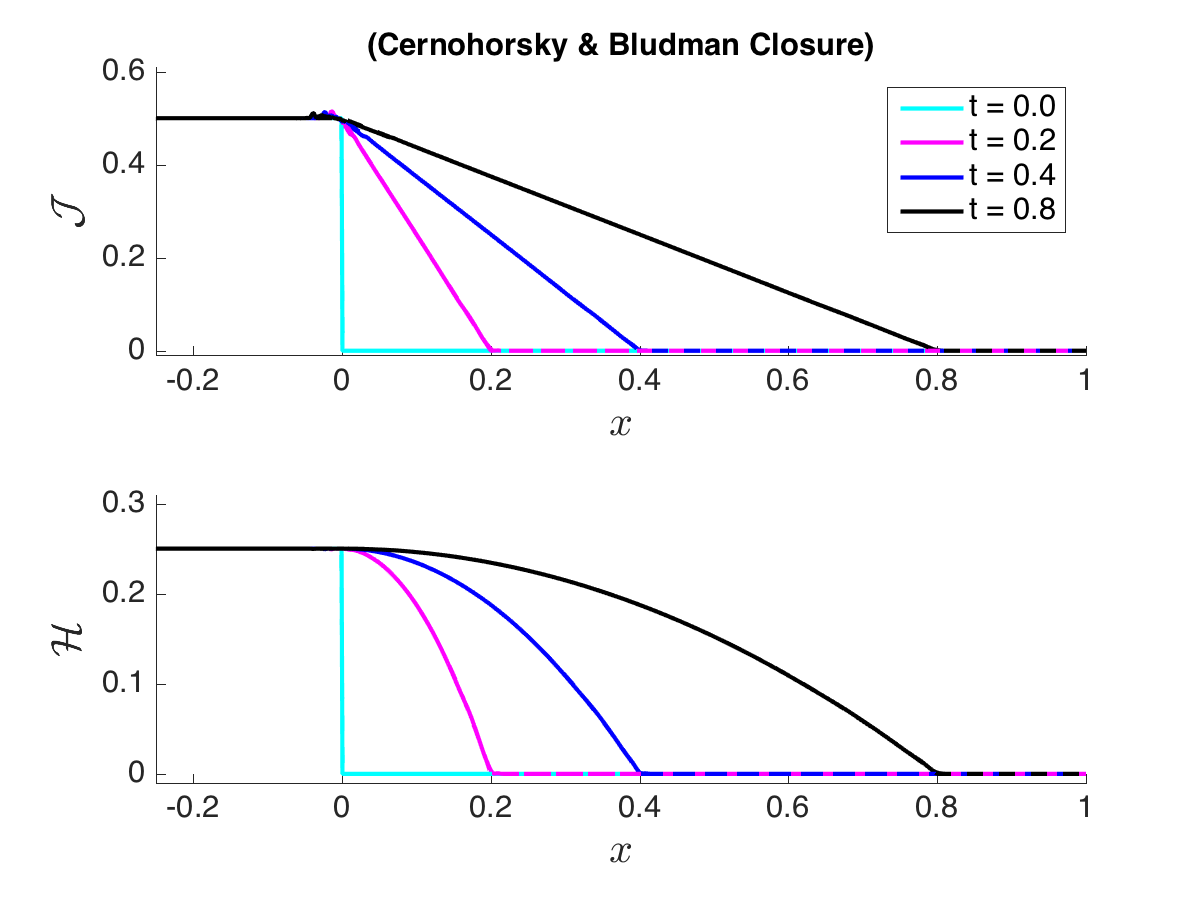
\includegraphics[width=0.485\textwidth]{figures/PackedBeam_ME_CB} &
    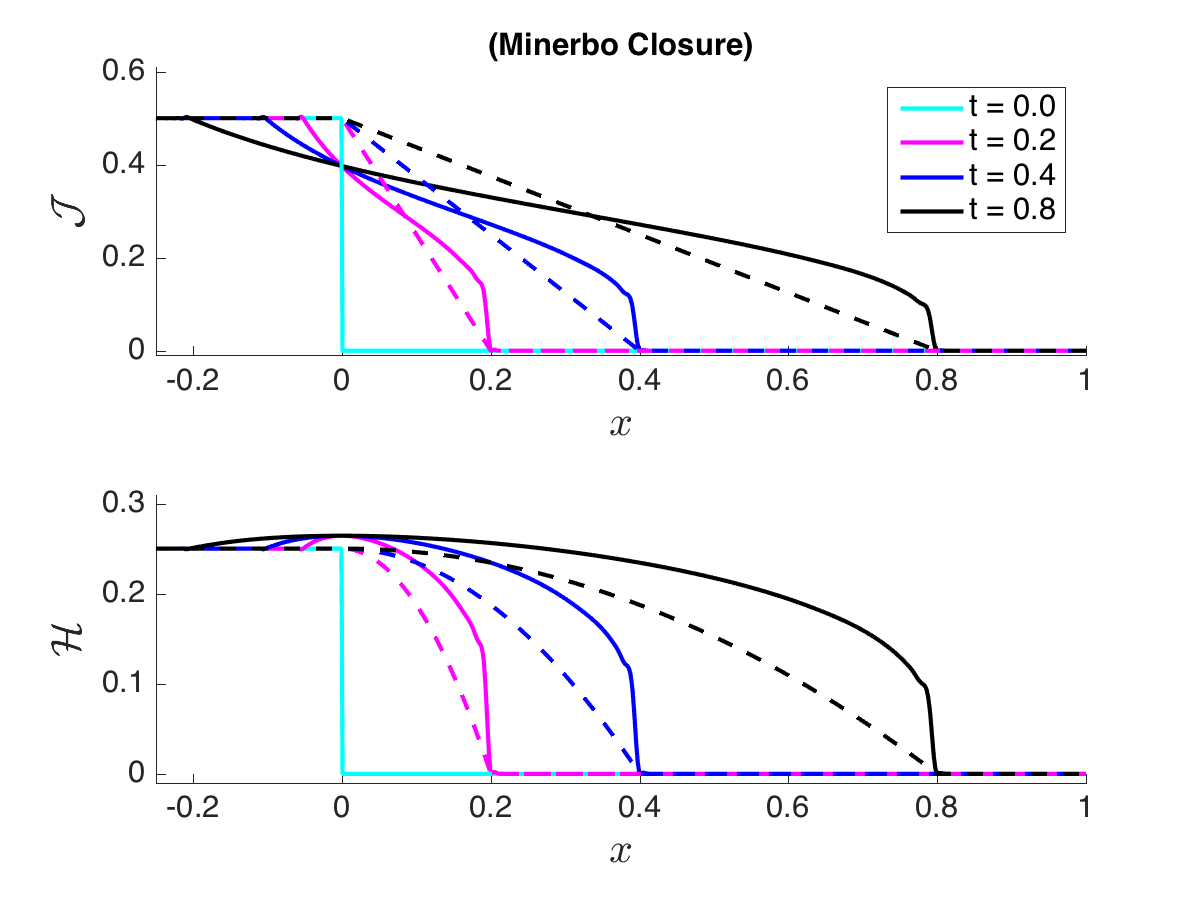
\includegraphics[width=0.485\textwidth]{figures/PackedBeam_ME_MI}
  \end{tabular}
   \caption{Numerical results from the packed beam problem at various times: $t=0$ (cyan), $t=0.2$ (magenta), $t=0.4$ (blue), and $t=0.8$ (black).  Results obtained with the Cernohorsky \& Bludman closure are displayed in the left panels, while results obtained with the Minerbo closure are displayed in the right panels.  The analytical solution (dashed lines) is also plotted.}
  \label{fig:PackedBeam}
\end{figure}

As can be seen in Figure~\ref{fig:PackedBeam}, with the CB closure the numerical solution obtained with the two-moment model tracks the analytic solution well, while with the Minerbo closure the numerical solution deviates substantially from the analytic solution.  
With the Minerbo closure, the solution also evolves outside the realizable domain for Fermi-Dirac statistics.  

In the left panel in Figure~\ref{fig:PackedBeam_Realizability} we plot $\gamma(\vect{\cM})=\big(1-\cJ\big)\,\cJ-|\vect{\cH}|$ versus position for various times.  
With the Minerbo closure, $\gamma(\vect{\cM})$ becomes negative in regions of the computational domain (dashed lines), while $\gamma(\vect{\cM})$ remains positive for all $x$ and $t$ the CB closure.  
In the right panel of Figure~\ref{fig:PackedBeam_Realizability} we plot the numerical solutions in the $(\cH,\cJ)$-plane.  
Initially, the moments are located in two points: $\vect{\cM}_{\mbox{\tiny L}}$ and $\vect{\cM}_{\mbox{\tiny R}}$, for $x\le0$ and $x>0$, respectively.  
For $t>0$, the solutions trace out curves in the $(\cH,\cJ)$-plane, connecting $\vect{\cM}_{\mbox{\tiny L}}$ and $\vect{\cM}_{\mbox{\tiny R}}$.  
With the CB closure, the solution curve (blue points) follows the boundary of the realizable set $\cR$ defined in Eq.~\eqref{eq:realizableSet} (cf. black line in Figure~\ref{fig:PackedBeam_Realizability}).  
With the Minerbo closure (magenta points), the solution follows a different curve --- outside the realizable domain for distribution functions bounded by $f\in[0,1]$, but inside the realizable domain of positive distributions (cf. red line in Figure~\ref{fig:PackedBeam_Realizability}).  
We have also run this test using the algebraic maximum entropy closure of Larecki \& Banach \cite{lareckiBanach_2011} and the simpler Kershaw-type closure in \cite{banachLarecki_2017a}.  
The numerical solutions obtained with both of these closures follow the analytic solution well, and remain within the realizable set $\cR$.  
We point out that simply using the realizability-preserving limiter described in Section~\ref{sec:limiter} with the Minerbo closure does not result in a realizability-preserving scheme for Fermi-Dirac statistics because of the properties of this closure discussed in Section~\ref{sec:algebraicClosure}, and plotted in the lower right panel of Figure~\ref{fig:MabWithDifferentClosure}.  

\begin{figure}[h]
  \centering
  \begin{tabular}{cc}
    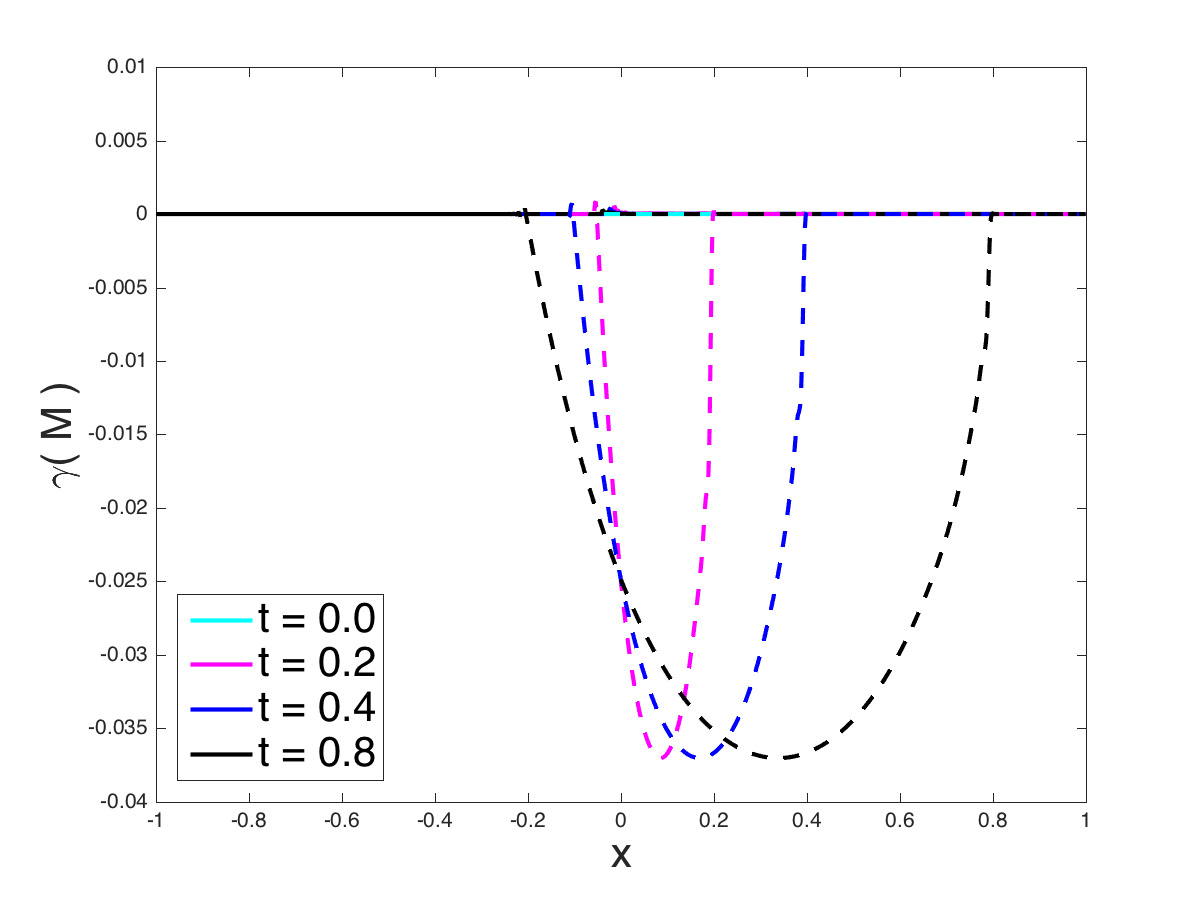
\includegraphics[width=0.485\textwidth]{figures/PackedBeam_Realizability} &
    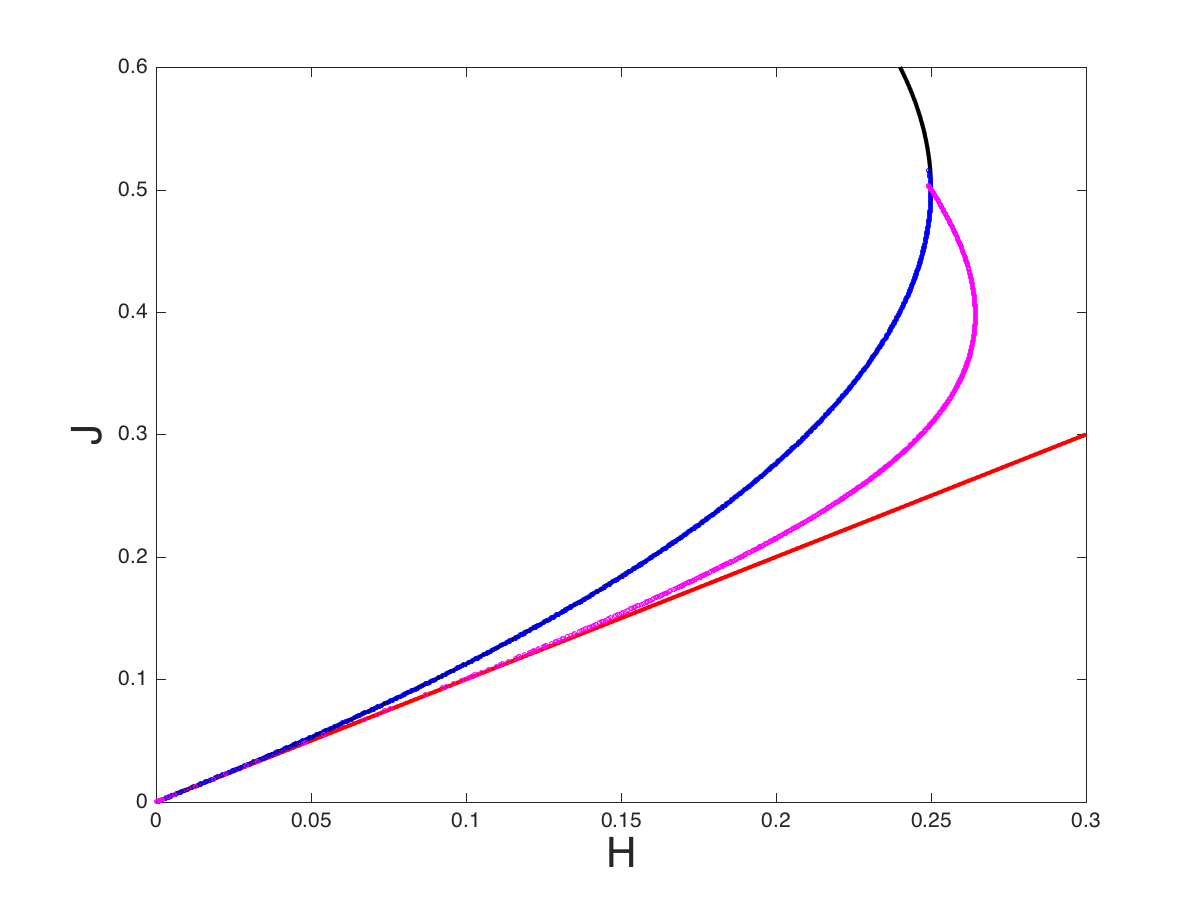
\includegraphics[width=0.485\textwidth]{figures/PackedBeam_RealizableDomain}
  \end{tabular}
   \caption{In the left panel, $\gamma(\vect{\cM})=(1-\cJ)\,\cJ-|\vect{\cH}|$ is plotted versus $x$ for various times in the packed beam problem: $t=0$ (cyan), $t=0.2$ (magenta), $t=0.4$ (blue), and $t=0.8$ (black).  Results obtained with the CB closure, which remain positive throughout the evolution, are plotted with solid lines, while results obtained with the Minerbo closure are plotted with dashed lines.  In the right panel, the moments are plotted in the $(\cH,\cJ)$-plane for the same times as in the left panel.  Results obtained with the CB and Minerbo closures are plotted in blue and magenta, respectively.  The solid black and red lines are contours where $(1-\cJ)\,\cJ=\cH$ and $\cJ=\cH$, respectively.}
  \label{fig:PackedBeam_Realizability}
\end{figure}

\subsection{Fermion Implosion}

The next test is inspired by line source benchmark (cf. \cite{brunner_2002,garrettHauck_2013}), which is a challenging test for approximate transport algorithms.  
The original line source test consists of an initial delta function particle distribution in radius $R=|\vect{x}|$; i.e., $f_{0}=\delta(R)/4\,\pi$.  
For $t>0$, a radiation front propagates in the radial direction, away from the initial source.  
Apart from capturing details of the exact transport solution, maintaining realizability of the two-moment solution is challenging.  

Here, a modified version of the line source --- dubbed \emph{Fermion Implosion},  designed to test the realizability-preserving properties of the two moment model for fermionic transport --- is computed on a two-dimensional domain with $D=\{\vect{x}\in\bbR^{2}:x^{1}\in[-1.28,1.28], x^{2}\in[-1.28,1.28]\}$.  
Instead of initializing with a delta function, we follow the initialization procedure in \cite{garrettHauck_2013}, and approximate the initial condition with an isotropic Gaussian distribution function.  
Morover, the initial distribution function is bounded $f_{\mbox{\tiny G},0}\in(0,1)$ and reaches a minimum in the center of the computational domain (hence implosion)
\begin{equation}
  f_{\mbox{\tiny G},0}
  =1-\max\Big[\,e^{-R^{2}/(2\,\sigma_{\mbox{\tiny G}}^{2})},10^{-8}\,\Big].  
\end{equation}
We set $\sigma_{\mbox{\tiny G}}=0.03$, and run this test to a final time of $t=1.0$.  
We run this test using a grid of $512^{2}$ elements, polynomials of degree $k=1$, and the SSPRK2 time stepping scheme; a second-order accurate scheme.  
(There are no collisions in this test; i.e., $\sigma_{\Ab}=\sigma_{\Scatt}=0$.)  
We present results using both the algebraic closure of Cernohorsky \& Bludman and the Minerbo closure.  

\begin{figure}[h]
  \centering
  \begin{tabular}{cc}
    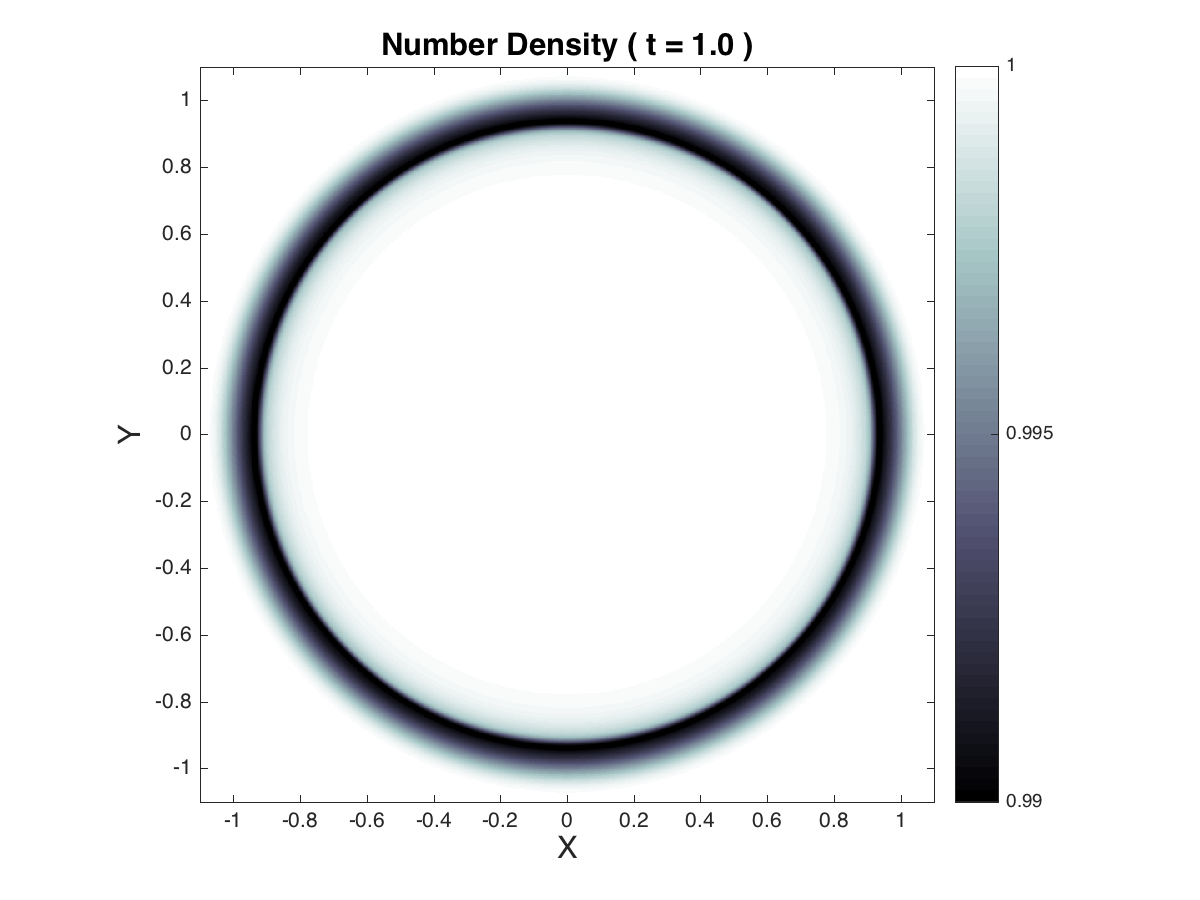
\includegraphics[width=0.495\textwidth]{figures/Implosion_Image} &
    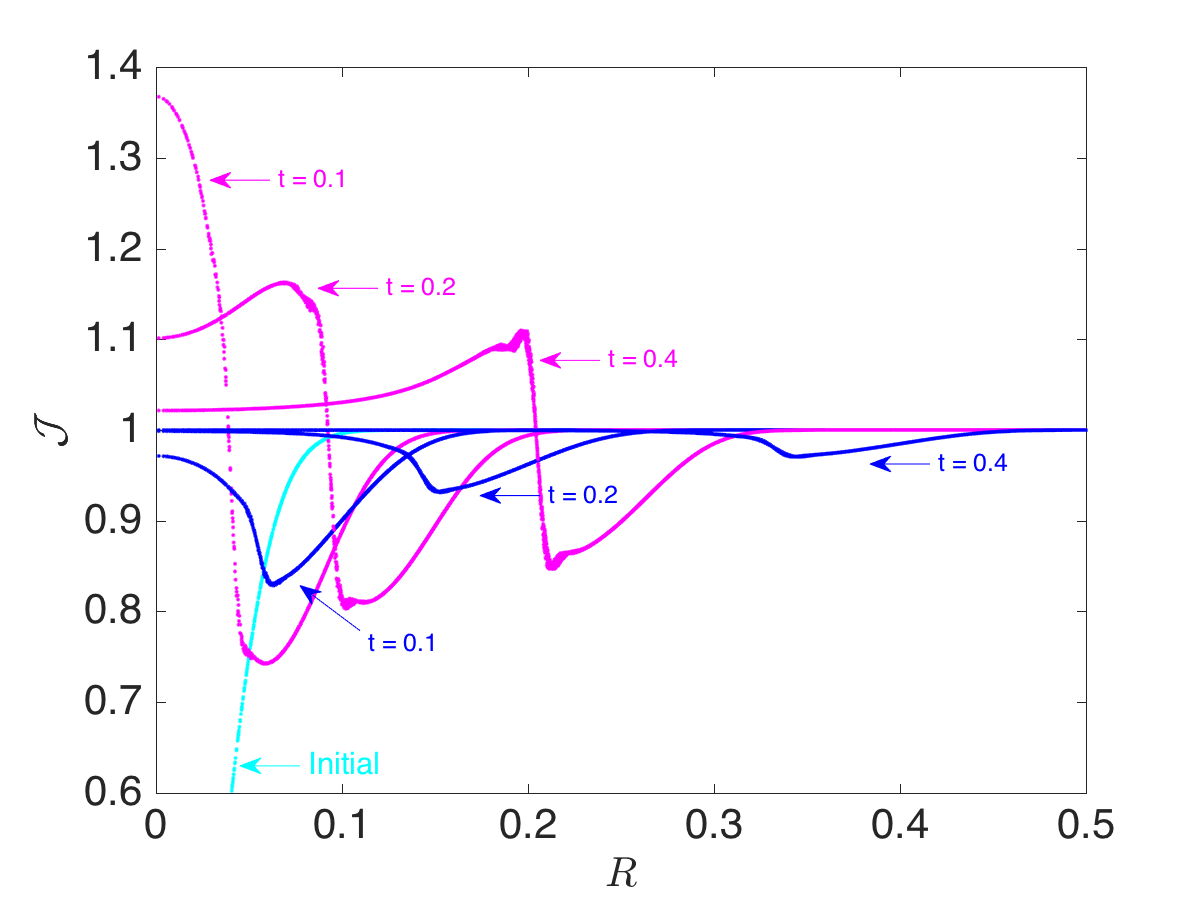
\includegraphics[width=0.495\textwidth]{figures/Implosion_Lineout} \\
    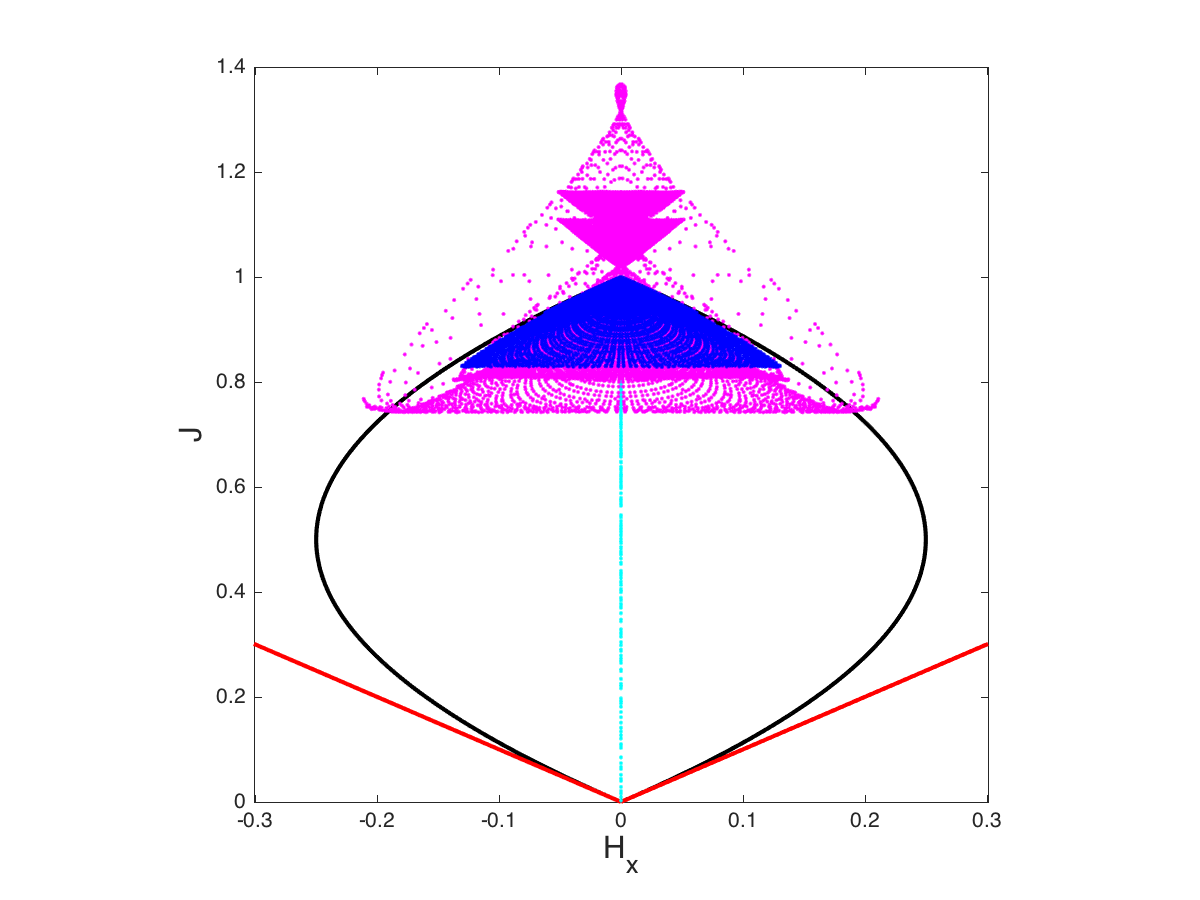
\includegraphics[width=0.495\textwidth]{figures/Implosion_RealizableDomain} &
    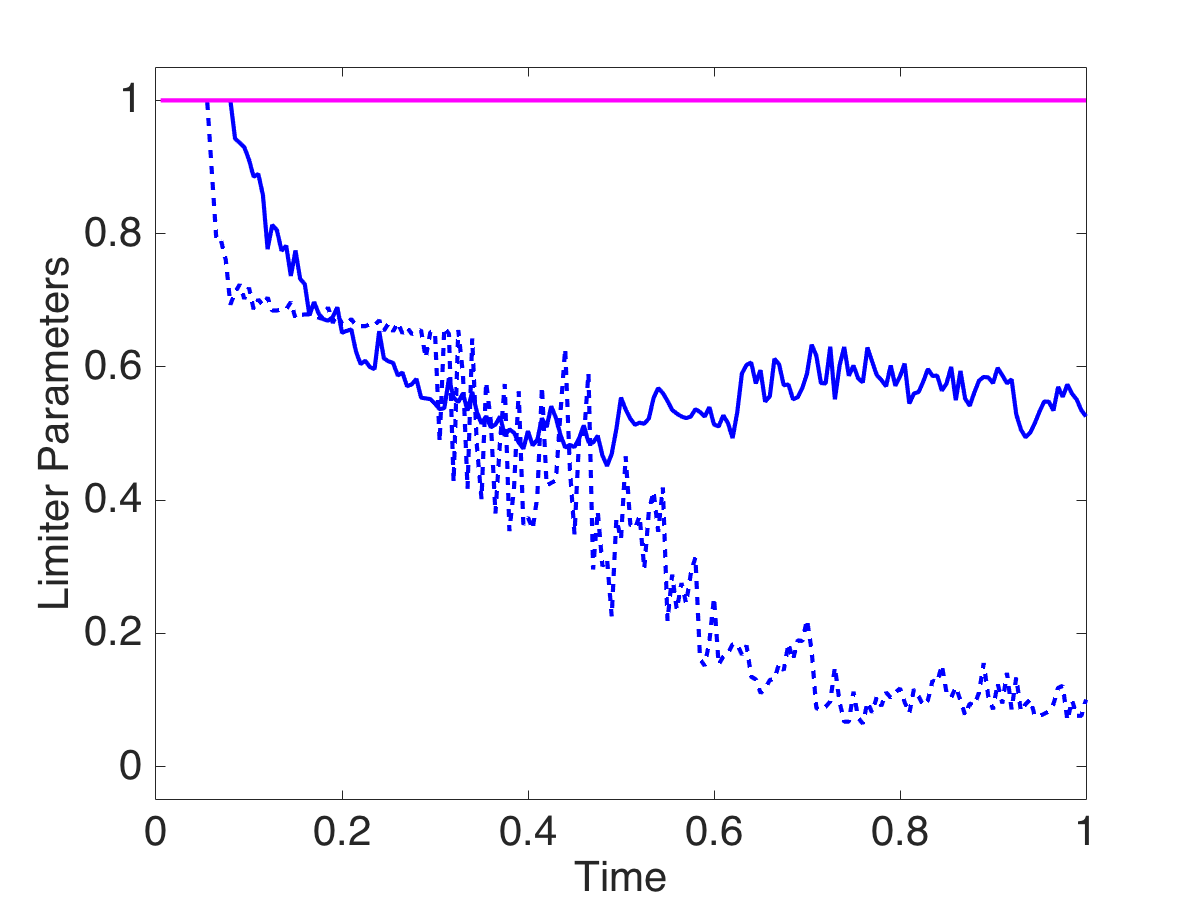
\includegraphics[width=0.495\textwidth]{figures/Implosion_LimiterParameters}
  \end{tabular}
   \caption{}
  \label{fig:Implosion}
\end{figure}

\subsection{Homogeneous Sphere}

The homogeneous sphere test (e.g., \cite{smit_etal_1997}) considers of a sphere with radius $R$.  
Inside the sphere (radius $<R$), the absorption opacity $\sigma_{\Ab}$ and the equilibrium distribution function $f_{0}$ are set to constant values.  
The scattering opacity $\sigma_{\Scatt}$ is set to zero in this test (i.e., $\xi=1$).  
Outside the sphere, the absorption opacity is zero.  
The steady state solution, obtained by solving the transport equation in spherical symmetry, is given by
\begin{equation}
  f_{\mbox{\tiny A}}(r,\mu)=f_{0}\,\big(1-e^{-\chi_{0}\,s(r,\mu)}\big),
  \label{eq:distributionHomogeneousSphere}
\end{equation}
where
\begin{equation}
  s(r,\mu)
  =\left\{
  \begin{array}{lll}
    r\,\mu+R\,g(r,\mu) & \mbox{if}\quad r<R, & \mu\in[-1,+1], \\
    2\,R\,g(r,\mu) & \mbox{if}\quad r \ge R, & \mu\in[(1-(R/r)^{2})^{1/2},+1], \\
    0 & \mbox{otherwise},
  \end{array}
  \right.
\end{equation}
and $g(r,\mu)=[1-(r/R)^{2}(1-\mu^{2})]^{1/2}$.  

\begin{figure}[h]
  \centering
  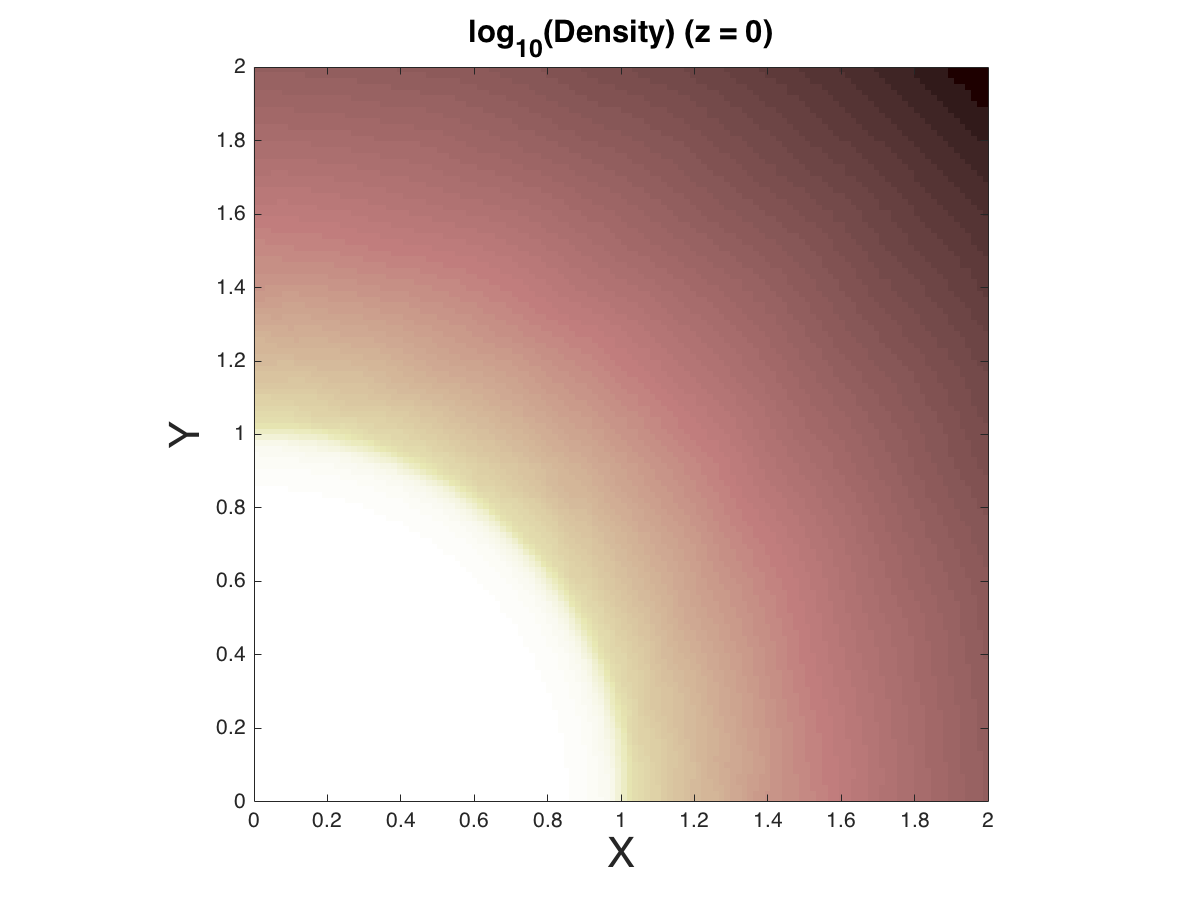
\includegraphics[width=1.0\textwidth]{figures/HomogeneousSphere_Resolution_3}
  \begin{tabular}{cc}
    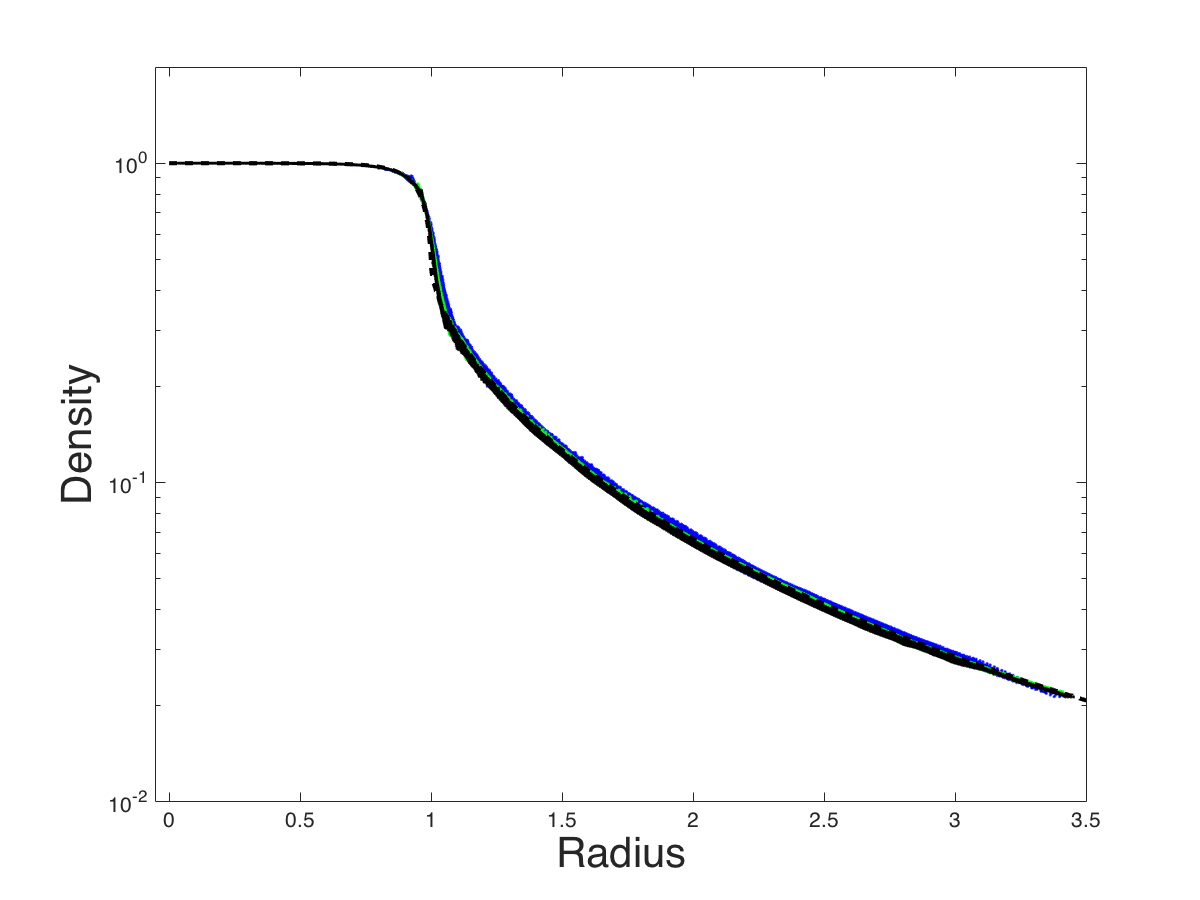
\includegraphics[width=0.5\textwidth]{figures/HomogeneousSphere_Resolution_1}
    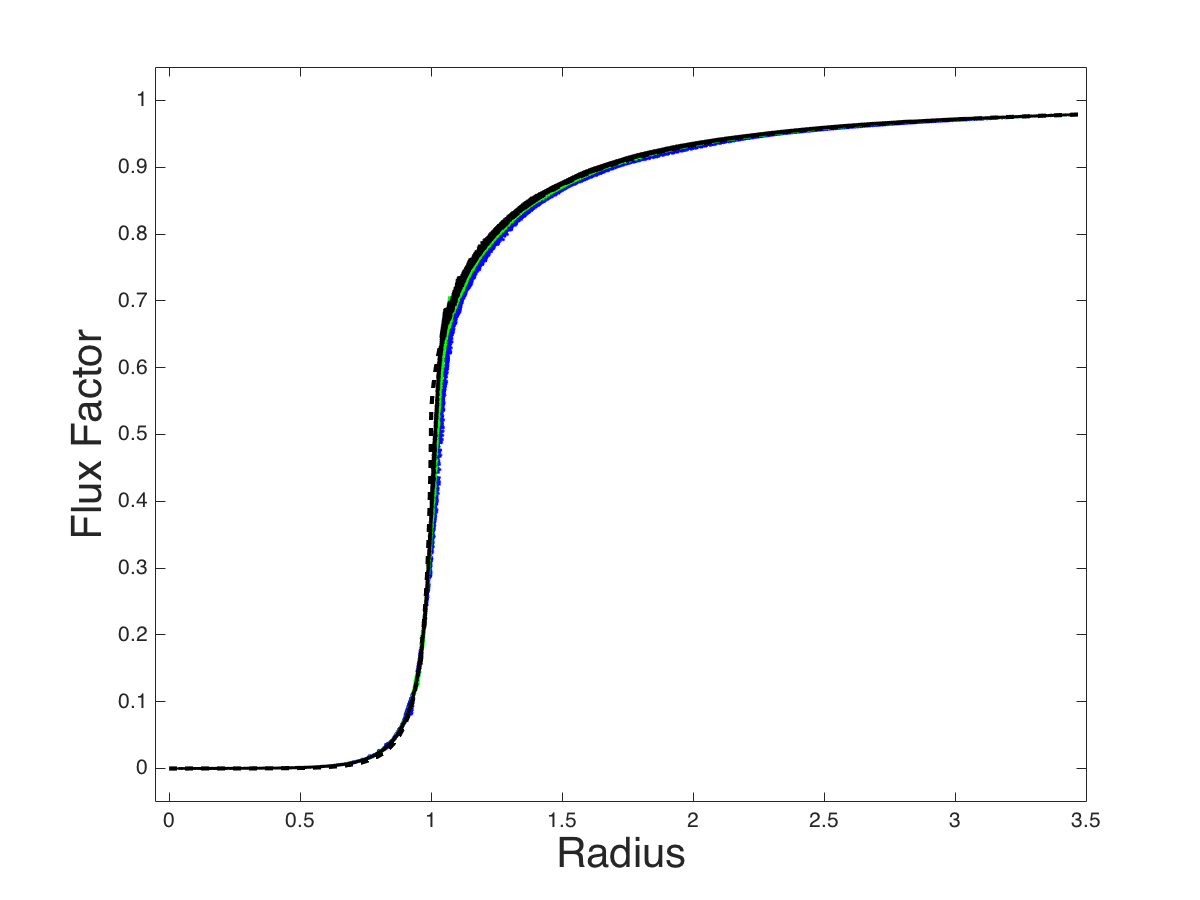
\includegraphics[width=0.5\textwidth]{figures/HomogeneousSphere_Resolution_2}
  \end{tabular}
   \caption{Homogeneous sphere problem: 32$^{3}$, 48$^{3}$, and 64$^{3}$}
  \label{fig:HomogeneousSphere_Resolution}
\end{figure}